\chapter{Literature Review and Gap Analysis}\label{literature}
Research on insider threat detection has expanded over time, and the creators of the research have used various methods, from rule-based to statistical models of the old era to modern ML, DL, and hybrid methods. The systematic overview of the existing approaches with a focus on the timeline of the techniques and their contribution is examined from different angles, such as ML, DL, graph, and hybrid approaches, to clarify the work.

\subsection{Machine Learning Approaches}
The main goal of the implementation was to find insider threats using ML methods, which can make sense of complex behavioral patterns in large datasets.  B. Bin Sarhan and N. Altwaijry \cite{bin2022insider} presented dimensionality reduction through Principal Component Analysis (PCA) and classification via Support Vector Machine (SVM), in addition to anomaly detection techniques.  The existing approaches claim superior accuracies, but without performing any validation experiments, the reliability of those cannot be considered as an effective solution due to poor generalization. P. Manoharan et al. \cite{manoharan2023insider} proposed a supervised framework using an ML algorithm with higher accuracy, but the false positive rate is higher. However, the method wasn't tested on real-world data with noise to make sure it worked.


 Wall et al. \cite{wall2021bayesian} proposed a probabilstic bayesian method  for superior assumptions based on inputs. Duc C. Le et al. \cite{le2020analyzing} used Random Forest (RF) on CERTr5.2 and yielded superior results with only drawback being neglecting  the dynamic temporal consideration, resulting in a limited dependecies. Sivakrishna \cite{sivakrishna2025efficient} and P. Chattopadhyay et al. \cite{chattopadhyay2018scenario} combined supervised algorithms with CERTr4.2 in an effort to model typical anomalous behavior for superior classification accuracy. F. Janjua et al. \cite{janjua2020handling} performed a comparative analysis of several ML classifiers utilizing a limited TWOS dataset, thereby making their results predominantly irrelevant to broader, real-world scenarios.

\begin{table}[!ht]
\caption{Summary of Machine Learning Approaches for Insider Threat Detection}\label{tbl1}
\begin{tabular}{   p{3cm}p{2cm}  p{3cm}  p{4cm} }
\toprule
\textbf{References} & \textbf{Dataset} & \textbf{Technique}  & \textbf{Limitations} \\
\midrule
 

B. Bin Sarhan and N. Altwaijry \cite{bin2022insider} & CERTr4.2 & SVM, Anomaly Detection, PCA. &  Lack of temporal modeling and risk of overfitting. \\
\cmidrule(lr){1-4}
A. Singh et al. \cite{singh2024improving} & CERTr4.2 & Isolation Forest (IF) & May lose legitimate behavior info due to cost sensitive adjustments (class imbalance).\\
\cmidrule(lr){1-4}

P. Manoharan et al. \cite{manoharan2023insider} & CERTr4.2 & Supervised algorithms &  Lacks temporal framework of evolving behaviors. \\
\cmidrule(lr){1-4}


 Wall et al. \cite{wall2021bayesian}& CERTr4.1 & Bayesian Network & Features like email and website content were not considered. \\
\cmidrule(lr){1-4}

Duc C. Le et al. \cite{le2020analyzing}& CERTr5.2 & RF & Ensemble lacks transparency. \\
%%%%%%%%%%%%%%%%%%%%%%%%%%%%%%%%%%
\cmidrule(lr){1-4}
P. Chattopadhyay et al. \cite{chattopadhyay2018scenario}& CERTr4.2 & Supervised algorithms & Lacks representation of typical anomalous behavior, reducing classification accuracy. \\
\cmidrule(lr){1-4}

F. Janjua et al. \cite{janjua2020handling}& TWOS & AdaBoost, NB, LR, KNN, SVM & Class imbalance issues and lack of diversity. \\
\bottomrule
\end{tabular}

\end{table}


\subsection{Deep Learning Approaches}
Several deep learning-based methods have been explored for insider threat detection, each with its strengths and limitations. F. Yuan et al. \cite{yuan2019attention} used an Long Short-Term Memory (LSTM) framework on the CERTr4.2 dataset. But here, the framework has faced challenges in handling different sequence lengths, leading to degraded performance and increased false alarms \cite{sivakrishna2023aubit}. Similarly, R. Nasir et al. \cite{nasir2021behavioral} employed an LSTM Autoencoder. The detection relied solely on role- and session-based traits, limiting its ability to capture more complex insider behaviors. Gupta et al. \cite{gupta2021lio} implemented LSTM on multiple datasets, including New Standard Link-Knowledge Discovery and Data Mining (NSL-KDD), Coburg Intrusion Detection Data Sets-001 (CIDDS-001), and Canadian Institute for Cybersecurity Intrusion Detection System 2017 (CICIDS2017), but the one-vs-one classification technique introduced complexity in both implementation and tuning. S. Yuan et al. \cite{yuan2020few} adopted a Few-shot Fine-tuning framework for CERTr4.2 and Universal Module (UMD) Wikipedia datasets. the framework was limited to binary anomaly detection, lacking fine-grained classification. H. Liu et al \cite{liu2025ripple2detect} introduced the Bidirectional Encoder Representations from Transformers (BERT) approach, inflexible with unknown patterns.


Deep neural networks have also been used for insider threat detection. M. N. Al-Mhiqani et al. \cite{al2021integrated} proposed an Adaptive Synthetic-Deep Neural Network (AD-DNN) framework on CERTr4.2. This framework struggled with high-dimensional, sparse user behavior data, making it less effective in real-world scenarios. Using image classification techniques, v. Rohini et al. \cite{rohini2024insider, randive2023efficient} focus on detecting insider threats. The CERTr4.2 dataset was utilized, and data augmentation was applied to address class imbalance. The study evaluates the effectiveness of the Residual Network (ResNet50) framework for insider threat detection. Image-based deep-learning approaches have also been explored. R. Gayathri et al. \cite{gayathri2020image} utilized Visual Geometry Group (VGG19) on CERTr4.2, but Convolutional Neural Network (CNN) pooling operations resulted in the loss of important features, reducing detection accuracy. K. Randive et al. \cite{randive2023mwcapsnet} developed Multi-level Wavelet Capsule Network (MWCapsNet), combining MW decomposition with CapsNet on CERTr4.2 and r5.2, but the framework was computationally intensive, requiring significant resources for training and inference.

The lack of interpretability in these approaches makes it challenging for security analysts to understand. Deep learning approaches, as shown in Table \ref{tbl2}, have gained traction in the detection of insider threats due to their ability to framework complex patterns and also face challenges with data sparsity and high-dimensional feature spaces.

\begin{table}[!ht]
\caption{Summary of Deep Learning Approaches for Insider Threat Detection}
\begin{tabular}{  p{2.5cm} p{3cm}  p{2cm}  p{4.5cm} }
\toprule
\textbf{References} & \textbf{Dataset} & \textbf{Technique}  & \textbf{Limitations} \\
\midrule
 R. Nasir et al. \cite{nasir2021behavioral}& CERTr4.2 & LSTM-Autoencoder & Autoencoder lacks transparency in prediction reasoning. \\
\cmidrule(lr){1-4}
 N. Gupta et al. \cite{gupta2021lio} & NSL-KDD, CIDDS-001, \& CICIDS2017 & LSTM & Difficulty in scalability for multiclass. \\
\cmidrule(lr){1-4}
 S. Yuan et al.  \cite{yuan2020few}& CERTr4.2 \& UMDWikipedia Dataset & Few-shot Fine-tuning & Limited to distinguishing anomalies from normal samples, not fine-grained anomaly classification. \\
\cmidrule(lr){1-4}
 H. Liu et al. \cite{liu2025ripple2detect} & CERTr4.2 \& r5.2 & BERT & Poor adaptability to new behaviors.\\

\cmidrule(lr){1-4}
 M. N. Al-Mhiqani et al. \cite{al2021integrated}& CERTr4.2 & AD-DNN & Struggles with complex, high-dimensional, and sparse user behavior data. \\
\cmidrule(lr){1-4}
V Rohini et al. \cite{rohini2024insider}& CERTr4.2& ResNet & Image conversion lacks behavioral fidelity. \\
\cmidrule(lr){1-4}
 R. Gayathri et al. \cite{gayathri2020image}& CERTr4.2 & VGG19 & Loss of context over time. \\
\cmidrule(lr){1-4}
K. Randive and M. Ramasundaram \cite{randive2023mwcapsnet} & CERTr4.2\& r5.2 & MWCapsNet & MW decomposition with CapsNet is complex and resource-intensive. \\
\bottomrule
\end{tabular}

\label{tbl2}
\end{table}


\subsection{Graph Neural Network Approaches}
Graph-based approaches have been used for insider threat detection because they can analyze relationships between different activities and users. 
However, these methods also have some challenges. J. Xiao et al. \cite{xiao2022robust} introduced the Deep Temporal Graph Infomax (DTGI) framework using the CERTr6.2 dataset which required more features in the weighted edges to improve detection accuracy. 

Other researchers have tried different graph-based techniques to detect insider threats. K. Fei et al. \cite{fei2022graph} introduced Log2Graph based on Graph Convolution Neural Network (GCN) for analyzing Los Alamos National Laboratory (LANL) data. It was useful for detecting malicious users and hosts, but failed to detect lateral movements, which are crucial for identifying hidden threats. Some studies focused on improving detection by using deep graph approaches. X. Li et al. \cite{li2023high} developed the Dual-Domain GCN (DD-GCN) framework on CERTr4.2 and r6.2. This framework needed a large amount of data for training and sometimes made incorrect predictions, leading to false positives. Similarly, J. Jiang et al. \cite{jiang2019anomaly} used a GCN-based framework on CERTr4.2, but it lacks of labeled training data and does not consider important connections between different activities.  

As summarized in Table \ref{tbl3}, graph-based approaches are useful for understanding how different users and activities are connected in insider threat detection. They help in revealing concealed patterns and identifying abnormal behavior. Nevertheless, these methods have challenges too, for instance, they can omit important information, require a large amount of data for training, and cannot easily follow changes in user behavior over time. 

\begin{table}[!ht]
\caption{Summary of Graph Neural Network Approaches for Insider Threat Detection}
\begin{tabular}{p{2.5cm}p{3cm}  p{2cm}  p{4.5cm} }
\toprule
\textbf{References} & \textbf{Dataset} & \textbf{Technique}  & \textbf{Limitations} \\
\midrule
P. Gao et al. \cite{gao2025deep} & CERTr6.2 & Graph Neural Network (GNN) & Assumes daily behavior snapshots, which may not capture fine-grained activities (e.g., Session-wise Preprocessing anomalies).\\
\cmidrule(lr){1-4}
 J. Xiao et al. \cite{xiao2022robust} & CERTr6.2& DTGI & Lack of explanation about edge semantics and dynamic weights \\
\cmidrule(lr){1-4}
 K. Fei et al. \cite{fei2022graph} & LANL & Log2Graph GCN & Focus on malicious users and hosts, missing lateral movements detection. \\
\cmidrule(lr){1-4}
 X. Li et al. \cite{li2023high}& CERTr4.2 \& r6.2& DD-GCN & Requires large data for training and may produce false positives. \\
\cmidrule(lr){1-4}
J. Jiang et al. \cite{jiang2019anomaly}& CERTr4.2& GCN & Lack of labeled samples and omitted structural relationships between entities. \\
\bottomrule
\end{tabular}

\label{tbl3}
\end{table}
\subsection{Hybrid Approaches}
Various hybrid methods have been formulated for insider threat detection to include the combination of different machine learning and deep learning techniques. 
L. Lin et al. \cite{lin2017insider} presented a Deep Belief Network One-Class SVM (DBN-OSCVM) model on CERTr4.2. This model was totally data-driven and didn't take into account user behavior, thus being very obscure in terms of the rationale behind the flagged activities. M. Singh et al. \cite{singh2023user} combined LSTM, Artificial Neural Network (ANN), and SVM for threat detection. While such a combination of techniques led to superior accuracy, it was still at a loss with sizeable datasets and sophisticated behavioral patterns, hence, scaling in the actual environment was infeasible.

P. Pal et al. \cite{pal2023temporal} investigated the stacking of LSTM and Stacked-Gated Recurrent Unit (GRU), A. M. Sivakrishna et al. \cite{sivakrishna2025efficient,sivakrishna2025temporal} presented XGBoost with Bayesian optimization and quantum neural networks with PCA on various CERT datasets (r4.2, r5.2, and r6.2). Deep learning models have achieved excellent performance, but the lack of interpretability makes it difficult to explain the rationale for the suspicion of the particular action. Duc C. Le et al. \cite{le2021anomaly} evaluated the performance of several anomaly detection methods (Autoencoder, IF, Lightweight On-Line Anomaly Detection (LODA), and Local Outlier Factor (LOF) in CERTr4.2 and r6.2. However, their novel framework was not supported by validation in real-world settings, thereby questioning its feasibility. W. Hong et al. \cite{hong2023graph} presented Residual Hybrid Network (ResHybnet), a hybrid method that integrates GNN and CNN. The framework was successful; however, they only employed a tiny fraction of the dataset, which may have constrained the detection of a broad range of threats.

These methods leverage the promise of combining different techniques for insider threat detection, the downsides with them being a number of daunting issues like scalability, interpretability, and applicability in the real world. The next research in this field should be in forming strategies that will not only be accurate and efficient but also provide an explanation.
As summarized in Table \ref{tbl4}, these approaches have contributed to improving insider threat detection, but they also highlight important challenges. Some approaches struggle with scalability, and others are difficult to interpret.


\begin{table}[!ht]
\caption{Summary of Hybrid Approaches for Insider Threat Detection}
\begin{tabular}{p{2.5cm}p{3cm}  p{2cm}  p{4.5cm} }
\toprule
\textbf{References} & \textbf{Dataset} & \textbf{Technique}  & \textbf{Limitations} \\
\midrule
L. Lin et al. \cite{lin2017insider} & CERTr4.2& DBN-OSCVM & Entirely data-driven, no understanding of user characteristics. \\
\cmidrule(lr){1-4}
 M. Singh et al. \cite{singh2023user}& CERTr4.2& LSTM-ANN-SVM & Scaling to large datasets and complex behaviors is challenging. \\
\cmidrule(lr){1-4}
 P. Pal et al. \cite{pal2023temporal} &  CERTr4.2, r5.2 \& r6.2& Stacked-LSTM, Stacked-GRU & Complex approachs can still be hard to interpret. \\
\cmidrule(lr){1-4}
 Duc C. Le et al.  \cite{le2021anomaly} & CERTr4.2 \& r6.2& Autoencoder, IF, LODA, and LOF & Lack of real-world experimental feedback. \\
\cmidrule(lr){1-4}
W. Hong et al. \cite{hong2023graph} & CERTr4.2& ResHybnet (GNN and CNN) & Only a subset of the dataset was used as features. \\
\bottomrule
\end{tabular}

\label{tbl4}
\end{table}

\subsection{Motivation for Using LNNs}
Insider threat detection employs machine learning paradigms, each appropriate to the availability of labeled data and the extent of user behavior. Supervised paradigms like SVM and RF are effective when labeled data are available to distinguish non-malicious from insider user behavior. They are prone to deteriorate, however, for performance in the case of class imbalance. Unsupervised paradigms like IF and PCA are best suited for anomaly detection in unlabeled data and are effective in discovering rare or new insider behavior. Semi-supervised paradigms, with a small number of labeled samples and an enormous amount of unlabeled data, have been shown to work best for realistic security scenarios where known instances of threats are limited. Although the paradigm of reinforcement learning has yet to be widely explored for this purpose, it possesses the ability to framework adaptive and sequential user behavior. Deep learning approaches like CNN, LSTM networks, and AEs offer robust mechanisms for learning high-dimensional and temporal patterns of behavior. Still, they are prone to suffer from a lack of explainability and high requirements for the scale of data. Graph-based paradigms of learning framework user–entity interactions for contextual anomaly detection, while hybrid approaches employ multiple paradigms for the purpose of performance enhancement, albeit at the cost of increased complexity.

\begin{figure}
    \centering
    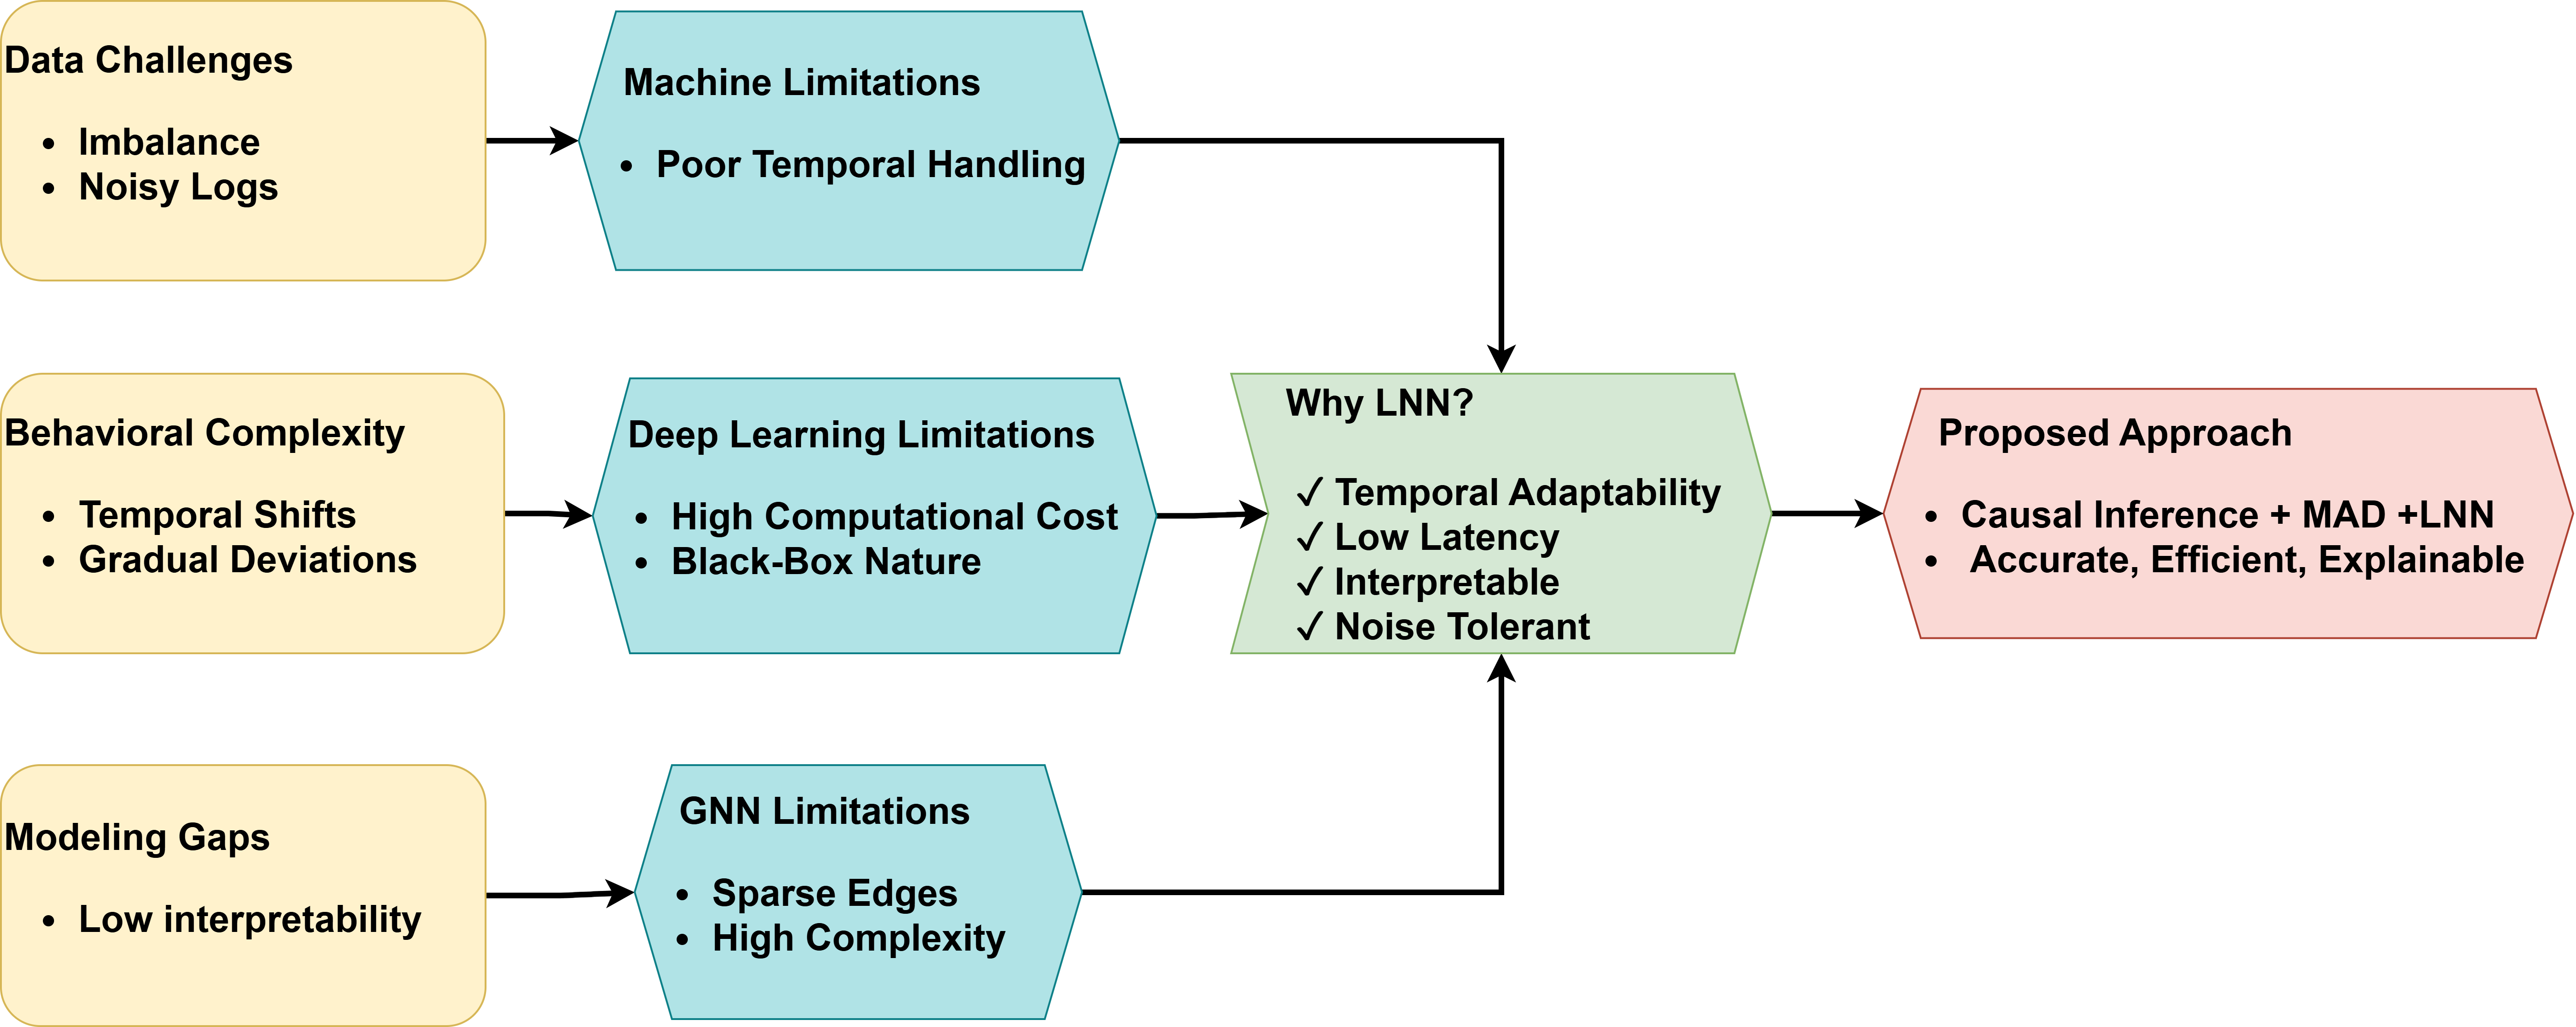
\includegraphics[width=1\linewidth]{figures/lnn_literature_survey_2_.png}
    \caption{Motivation for LNN}
    \label{lnn_suevey}
\end{figure}

The motivation and reasoning for embracing an LNN-based solution for insider threat detection problems shown in Figure \ref{lnn_suevey}. It starts with recognising major hindrances in three areas: data issues like imbalance and noisy logs, behavioral complexity with temporal changes and slow drifts, and modeling deficiencies characterised by low interpretability. These limitations result in constraints of conventional machine learning (poor time management), deep learning (expensive and black-box nature), and graph neural networks (sparse, high-level structures). To address this, LNN comes forth as a compelling alternative given its merits in temporal flexibility, low latency, interpretability, and robustness towards noise. The proposed method combines causal inference and MAD with LNN to provide a precise, efficient, and explainable detection system.


LNNs have emerged as a robust solution for noisy and time-varying settings with state-of-the-art performance in tasks ranging from time-series forecasting \cite{akpinar2025novel, hasani2021liquid}, signal classification \cite{cantini2025exact}, biomedical diagnosis and temporal knowledge inference \cite{han2025robust}, wireless communications \cite{wang2024robust}. Their ability to dynamically adapt to evolving inputs and framework continuous-time behaviors through differential equations makes them especially well-suited to approach the dynamic nature of insider threats. LNNs stand apart from traditional approaches in that they run at low computational cost, can process noisy or missing input streams, and preserve temporal memory, which is required for keeping track of real-time behavior. These features make them especially well-suited to insider threat detection, where subtle changes in behavior over time require accurate, adaptive responses.

The supervised learning strategy in this study, since pre-labeled user behavior between malicious and non-malicious is given in the CERTr4.2 dataset. This permits precise testing and training of classification approaches. Yet, conventional supervised approaches are temporally rigid and interpretable, both essential while insider threats unfolding over time and being driven by contextual and causal reasons. To overcome these issues, introduced a new approach, MAD based LNN, which combines LNNs' temporal reasoning powers with logical and causal interpretability. This framework permits strong, real-time insider threat detection even in noisy, imbalanced, or partially observable behavioral data settings.
